%%%%%%%%%%%%%%%%%%%%%%%%%%%%%%%%%%%%%%%%%%%%%%%%%%%%%%%%%%%%%%%%%%%%%%%%%%%%%%%%%%%%%%%%%
% Template de l'elaboració de TFG del Grau en informàtica de la Universitat de Girona (udg.)
% basat en https://github.com/matteodelucchi/ZHAW_thesis-template
%
% This template is based on previous works by:
% Steve Gunn (http://users.ecs.soton.ac.uk/srg/softwaretools/document/templates/)
% Sunil Patel (http://www.sunilpatel.co.uk/thesis-template/)
% Matteo Delucchi (https://github.com/matteodelucchi/ZHAW_thesis-template)
%
% University specific changes were made by:
%  Robert Martí (robert.marti@udg.edu)
% 
% Template license:
% CC BY-NC-SA 3.0 (http://creativecommons.org/licenses/by-nc-sa/3.0/)
%%%%%%%%%%%%%%%%%%%%%%%%%%%%%%%%%%%%%%%%%%%%%%%%%%%%%%%%%%%%%%%%%%%%%%%%%%%%%%%%%%%%%%%%%

%----------------------------------------------------------------------------------------
% DOCUMENT SPECIFICATION
%----------------------------------------------------------------------------------------
\documentclass[
    11pt,                      % Default font size
    %oneside,                  % One-side binding. Default: Two-side binding / alternating margins
    catalan,                   % Language. Feu servir english per anglès
    singlespacing,             % Spacing option: singlespacing, onehalfspacing or doublespacing
    %nolistspacing,            % Set spacing in lists to single
    %draft,                    % Enable draft mode: no pictures, no links, overfull hboxes indicated
    liststotoc,               % Include list of figures/tables/etc in the table of contents
    %toctotoc,                 % Include the main table of contents to the table of contents
    parskip,                  % Add vertical space between paragraphs
    %nohyperref,               % Disable links in the entire document
    headsepline,               % Show a horizontal line under the header
    %chapterinoneline,         % Place the chapter title and chapter number on one line
    consistentlayout,          % Have the same layout for special chapters: 
                               % declaration, abstract and acknowledgements
]{MastersDoctoralThesis}

% Uncomment the following lines to only include a subset of chapters.
% This is useful for long documents, as typesetting takes a bit of time
%\includeonly{
%    Front/titlepage,
%    Front/imprint,
%    Front/abstract,
%    %Front/declaration,
%    %Front/acknowledgements,
%    %Front/symbols,
%    Chapters/Chapter1,
%    %Chapters/Chapter2
%    }


%----------------------------------------------------------------------------------------
% PREAMBLE: PACKAGES AND CONFIGURATIONS
%----------------------------------------------------------------------------------------
% !TEX root = main.tex

%----------------------------
%   Fonts and characters
%----------------------------

% Support for special characters
\usepackage[utf8]{inputenc}    % Specify input encoding
\usepackage[T1]{fontenc}       % Specify font encoding
\usepackage{xurl}              % Allow line breaking in URLs at any character
\usepackage[hidelinks,breaklinks]{hyperref} % Clickable links without borders
\renewcommand{\_}{\textunderscore\allowbreak} % Allow breaking after underscores in texttt
\renewcommand{\_}{\textunderscore\allowbreak} % Allow breaking after underscores in texttt

% Set main fonts
% Fonts catalogue: https://tug.org/FontCatalogue/
\usepackage{mathpazo}          % Use the Palatino font by default
\usepackage{amsmath}
\usepackage[framemethod=TikZ]{mdframed}
\usepackage{translator}           % Required for math environments (cases, text, etc.)
\usepackage{beramono}          % Override the monospace/typewriter font

% UdG title font
% Try to load Georgia 
% Loading OTF or system fonts is possible with XeLaTeX.
% If the document is compiled using pdfLaTeX, resort 
\usepackage{ifxetex}
\ifxetex
    \usepackage{fontspec}
    \newfontfamily\udgtitlefont{Georgia}
\else
    \newcommand{\zhawtitlefont}{\scshape}
\fi

%\usepackage[scaled]{helvet}

%----------------------------
%   Environments
%----------------------------

\usepackage{caption}           % Customized caption
\usepackage{subcaption}        % Subfigure captions
\usepackage{float}             % Required for [H] figure placement
\usepackage{makecell}          % Per-cell formatting in tables (\makecell)
\usepackage{pdfpages}          % Required to include PDF files/graphics (\includepdf)

\usepackage{todonotes}         % Introduces the command \todo
\setlength{\marginparwidth}{2.5cm} % Adjust this if the todo notes are out of margins

\usepackage{pgfgantt}          % For Gantt charts
\usepackage{tikz}              % Required for creating graphics (timeline)
\usetikzlibrary{shapes, arrows}

% Create boxes as follows:
% \begin{colorbox}{red}{2}
\usepackage{tcolorbox}
\tcbuselibrary{breakable, skins} % Enable breakable boxes
\newtcolorbox{textbox}[2]{
    arc=3pt,
    boxrule=#2pt,
    colback=#1!25!white,
    width=\textwidth,
    halign=justify,
    valign=center,
    colframe=#1!75!black,
    breakable, % Allow box to break across pages
    enhanced   % Required for breakable to work optimally
}

\newtcolorbox{reflectionbox}{
    colback=white,
    colframe=gray!50,
    boxrule=0pt,
    leftrule=3pt,
    arc=0pt,
    outer arc=0pt,
    left=10pt,
    right=10pt,
    top=5pt,
    bottom=5pt,
    fontupper=\itshape\small
}

%----------------------------
%   Colors
%----------------------------

% Set up colors
\usepackage[table]{xcolor}
% UdG Blue: Pantone 2945 U / R0 G20 B137
\definecolor{udgblue}{rgb}{0.00, 0.07, 0.54}
% Colors related to code listings
\definecolor{codegreen}{rgb}{0,0.6,0}
\definecolor{codegray}{rgb}{0.5,0.5,0.5}
\definecolor{codepurple}{rgb}{0.58,0,0.82}
\definecolor{codebackground}{rgb}{0.93,0.94,0.95}

%----------------------------
%   Code listings
%----------------------------

% Setup code listings
\usepackage{listings}
\lstdefinestyle{mystyle}{
    commentstyle=\color{codegreen},
    keywordstyle=\color{magenta},
    numberstyle=\tiny\color{codegray},
    stringstyle=\color{codepurple},
    basicstyle=\ttfamily\footnotesize,
    breakatwhitespace=false,
    breaklines=true,
    columns=fullflexible,
    keepspaces=true,
    numbers=left,
    numbersep=5pt,
    showspaces=false,
    showstringspaces=false,
    showtabs=false,
    tabsize=4,
    % Support for Catalan/Spanish accents in code blocks
    literate={à}{{\`a}}1
             {è}{{\`e}}1
             {é}{{\'e}}1
             {í}{{\'i}}1
             {ò}{{\`o}}1
             {ó}{{\'o}}1
             {ú}{{\'u}}1
             {ç}{{\c c}}1
             {·}{{\textperiodcentered}}1
             {ï}{{\"i}}1
             {ü}{{\"u}}1
             {Ñ}{{\~N}}1
             {ñ}{{\~n}}1
             {¿}{{?`}}1
             {¡}{{!`}}1
             {À}{{\`A}}1
             {È}{{\`E}}1
             {É}{{\'E}}1
             {Í}{{\'I}}1
             {Ò}{{\`O}}1
             {Ó}{{\'O}}1
             {Ú}{{\'U}}1
             {Ç}{{\c C}}1
             {á}{{\'a}}1
}
\lstset{style=mystyle}

% Envoltar els blocs de codi amb un fons sòlid de mdframed per evitar fissures
\mdfdefinestyle{codebox}{
    backgroundcolor=codebackground,
    linecolor=codebackground,
    innerleftmargin=5pt,
    innerrightmargin=5pt,
    innertopmargin=5pt,
    innerbottommargin=5pt,
    skipabove=10pt,
    skipbelow=10pt,
    roundcorner=0pt,
    splitbottomskip=2pt,
    splittopskip=2pt
}
\surroundwithmdframed[style=codebox]{lstlisting}

% Define Dart Language
\lstdefinelanguage{Dart}{
  keywords={typeof, new, true, false, catch, function, return, null, catch, switch, var, if, in, while, do, else, case, break, const, final, class, void, int, double, String, bool, Map, List, dynamic, async, await, Future, Stream},
  keywordstyle=\color{magenta}\bfseries,
  ndkeywords={class, export, boolean, throw, implements, import, this},
  ndkeywordstyle=\color{darkgray}\bfseries,
  identifierstyle=\color{black},
  sensitive=false,
  comment=[l]{//},
  morecomment=[s]{/*}{*/},
  commentstyle=\color{codegreen}\ttfamily,
  stringstyle=\color{codepurple}\ttfamily,
  morestring=[b]',
  morestring=[b]",
  morestring=[s]{'''}{'''},
  morestring=[s]{"""}{"""}
}

% Define JSON Language
\colorlet{punct}{red!60!black}
\definecolor{background}{HTML}{EEEEEE}
\definecolor{delim}{RGB}{20,105,176}
\colorlet{numb}{magenta!60!black}

\lstdefinelanguage{json}{
    basicstyle=\footnotesize\ttfamily,
    numbers=left,
    numberstyle=\scriptsize,
    stepnumber=1,
    numbersep=8pt,
    showstringspaces=false,
    breaklines=true,
    frame=lines,
    backgroundcolor=\color{background},
    literate=
     *{à}{{\`a}}1
      {è}{{\`e}}1
      {é}{{\'e}}1
      {í}{{\'i}}1
      {ò}{{\`o}}1
      {ó}{{\'o}}1
      {ú}{{\'u}}1
      {ç}{{\c c}}1
      {·}{{\textperiodcentered}}1
      {ï}{{\"i}}1
      {ü}{{\"u}}1
      {Ñ}{{\~N}}1
      {ñ}{{\~n}}1
      {¿}{{?`}}1
      {¡}{{!`}}1
      {À}{{\`A}}1
      {È}{{\`E}}1
      {É}{{\'E}}1
      {Í}{{\'I}}1
      {Ò}{{\`O}}1
      {Ó}{{\'O}}1
      {Ú}{{\'U}}1
      {Ç}{{\c C}}1
      {á}{{\'a}}1
      {0}{{{\color{numb}0}}}{1}
      {1}{{{\color{numb}1}}}{1}
      {2}{{{\color{numb}2}}}{1}
      {3}{{{\color{numb}3}}}{1}
      {4}{{{\color{numb}4}}}{1}
      {5}{{{\color{numb}5}}}{1}
      {6}{{{\color{numb}6}}}{1}
      {7}{{{\color{numb}7}}}{1}
      {8}{{{\color{numb}8}}}{1}
      {9}{{{\color{numb}9}}}{1}
      {:}{{{\color{punct}{:}}}}{1}
      {,}{{{\color{punct}{,}}}}{1}
      {\{}{{{\color{delim}{\{}}}}{1}
      {\}}{{{\color{delim}{\}}}}}{1}
      {[}{{{\color{delim}{[}}}}{1}
      {]}{{{\color{delim}{]}}}}{1},
}

% minted is an alternative code listing package. (See chapter 2)
% For it to run successfully, ensure the following:
% - the Python package Pygments. Install with the following command:
%       python -m pip install Pygments
% - pdflatex (or xelatex) is executed with the flag --shell-escape
%   If you are using a TEX editor, you can modify the typesetting 
%   command somewhere in the settings.
%\usepackage[outputdir=build]{minted}
%\usemintedstyle{xcode}
% For fancier coloring schemes, see here:
% https://tex.stackexchange.com/questions/585582
% One could also create an own style in Pygments
% https://pygments.org/docs/styles/#creating-own-styles

%----------------------------
%   References
%----------------------------

% Set up references
\usepackage[
    backend=biber,             % Use biber backend (an external tool)
    sorting=none,              % Enumerates the reference in order of their appearance
    style=numeric-comp         % Choose here your preferred citation style
]{biblatex}
\addbibresource{example.bib}   % The filename of the bibliography

% BibLaTeX URL breaking settings
\setcounter{biburllcpenalty}{7000}
\setcounter{biburlucpenalty}{8000}
\setcounter{biburlnumpenalty}{8000}
\usepackage[autostyle=false]{csquotes} 
                               % Required to generate language-dependent quotes 
                               % in the bibliography

%----------------------------------------------------------------------------------------
%   MARGIN SETTINGS
%----------------------------------------------------------------------------------------

\geometry{
    paper=a4paper,      % Change to letterpaper for US letter
    inner=2.5cm,        % Inner margin
    outer=3.8cm,        % Outer margin
    top=1.5cm,          % Top margin
    bottom=1.5cm,       % Bottom margin
    bindingoffset=.5cm, % Binding offset
    %showframe,         % Show the type block of the page
}
\setlength{\parskip}{1em}
\usepackage{enumitem}          % Layout control for list environments (e.g, itemize)
%\setlist{noitemsep}           % Suppress extra spaces between items
%\setlist{nosep}               % Suppress spaces before/after list environments



%----------------------------------------------------------------------------------------
% THESIS INFORMATION: MODIFY THIS SECTION!
%----------------------------------------------------------------------------------------

% The information below is used in the following parts:
% - Title page
% - Imprint
% - Abstract / Zusammenfassung
% - Meta information of PDF

\thesistitle{NUMEN: Assistent per a estudis numerològics. }             % Thesis title,              command: \ttitle
\thesistype{Projecte Final de Grau}             % Type of thesis (e.g. Master Thesis) \ttype
\thesisdocument{Memòria}
\thesisdate{Setembre 2025}                     % Date of submission                  \tdate
\keywords{numerologia, filosofia, automatització, pseudociència. }
                                        % Keywords for the thesis,            \keywordnames
\author{David Quintanilla Jimenez}             % Your name,                          \authorname
\degree{Grau en Enginyeria Informàtica} % Degree name,                        \degreename
\studyprogram{Grau en Enginyeria Informàtica} 
                                        % Study program                       \studyprog
% \studyprogramlink{https://www.zhaw.ch/en/lsfm/study/master/applied-computational-life-sciences/}
                                        % Link to study program               \studyproglink

\supervisorA{Marta Fort i Masdevall}       % Name of supervisor 1,               \supnameA
\supervisorAmail{e=mc2@udg.edu}         % Email address of supervisor 1,      \supmailA
\supervisorAweb{https://en.wikipedia.org/wiki/Albert\_Einstein}  %            \supwebA
\supervisorAinfo{                       % Formatted info about supervisor 1:  \supinfoA
    \supnameA\\
    Universitat de Girona\\
    Email: \href{mailto:\supmailA}{\supmailA}\\
    Web: \href{\supwebA}{Link}
}

% Keep empty if there is no supervisor 2: \supervisorB{}
\supervisorB{Isaac Newton}              % Name of supervisor 2,               \supnameB
\supervisorBmail{f=am@newton.com}       % Email address of supervisor 2,      \supmailB
\supervisorBweb{https://ca.wikipedia.org/wiki/Isaac_Newton}                  % \supwebB
\supervisorBinfo{                       % Formatted info about supervisor 2:  \supinfoB
    \supnameB\\
    University of Cambridge\\
    Email: \href{mailto:\supmailB}{\supmailB}\\
    Web: \href{\supwebB}{Link}
}

\university{University of Girona}
                                        % University name                     \univname
\universitycatalan{Universitat de Girona}
                                        % University, in German               \univnameger
\department{xxxxxxxxxxxxxxx} 
                                        % Department,                         \deptname

% % Links
\universitylink      {https://www.udg.edu/}                   % \univlink
% \universitylinkgerman{https://www.zhaw.ch/de/university/}                   % \univlinkger
% \departmentlink      {https://www.zhaw.ch/de/lsfm/}                         % \deptlink
% \institutelink       {https://www.zhaw.ch/en/lsfm/institutes-centres/icls/} % \instlink
% \grouplink           {https://www.zhaw.ch/en/lsfm/institutes-centres/icls/computational-health/} % \grplink



\AtBeginDocument{
\hypersetup{pdftitle=\ttitle} % Set the PDF's title to your title
\hypersetup{pdfauthor=\authorname} % Set the PDF's author to your name
\hypersetup{pdfkeywords=\keywordnames} % Set the PDF's keywords to your keywords
}

\begin{document}
\frontmatter                  % Roman page numbering for the pre-content pages
\pagestyle{plain}             % Default to the plain heading style until the thesis style 
                              % is called for the body content


%----------------------------------------------------------------------------------------
% TITLE PAGE AND IMPRINT
%----------------------------------------------------------------------------------------
\include{Front/titlepage}
\let\cleardoublepage\clearpage
\include{Front/imprint}




%----------------------------------------------------------------------------------------
% ABSTRACT
%----------------------------------------------------------------------------------------
%\include{Front/abstract}


%----------------------------------------------------------------------------------------
% ACKNOWLEDGEMENTS
%----------------------------------------------------------------------------------------
%\include{Front/acknowledgements}


%----------------------------------------------------------------------------------------
% LIST OF CONTENTS/FIGURES/TABLES PAGES
%----------------------------------------------------------------------------------------
% Comment out if any of the following is not needed:
\tableofcontents  % Add main table of contents
%\listoffigures    % Add list of figures
%\listoftables     % Add list of tables


%----------------------------------------------------------------------------------------
% ABBREVIATIONS / SYMBOLS
%----------------------------------------------------------------------------------------
%\include{Front/symbols}


%----------------------------------------------------------------------------------------
% DEDICATION
%----------------------------------------------------------------------------------------
% \dedicatory{For/Dedicated to/To my\ldots} 


%----------------------------------------------------------------------------------------
% THESIS CONTENT - CHAPTERS
%----------------------------------------------------------------------------------------
\mainmatter % Begin numeric (1,2,3...) page numbering
\pagestyle{thesis} % Return the page headers back to the "thesis" style

% Include the chapters of the thesis as separate files from the Chapters folder
% Uncomment the lines as you write the chapters

% !TEX root = ../main.tex

\chapter{Introducció, motivacions, propòsit i objectius del projecte}
\label{Chapter1}

\section{Introducció}
Aquest document presenta el desenvolupament tècnic de \textbf{NUMEN}, un sistema informàtic dissenyat per a l'automatització d'estudis numerològics complexos. El projecte aborda la transformació d'un procés manual, propens a errors i ineficiència, en una solució de programari robusta, escalable i precisa.

Addicionalment, el projecte transcendeix la simple eina de càlcul per oferir una estratègia de visibilitat externa mitjançant una plataforma pública. Aquesta vessant no només contextualitza els conceptes teòrics de la numerologia, sinó que està dissenyada per generar \textit{engagement}: presenta exemples reals d'estudis complets, ofereix una utilitat gratuïta (un "tastet") per al càlcul immediat del Camí de Vida —l'indicador base de la numerologia, que suposa una petita part del que és un estudi numerològic— i habilita un canal de comunicació directe amb el professional via WhatsApp, tancant així el cercle entre la curiositat de l'usuari i el servei expert.  A més, incorpora una gestió integral d'informes connectada a una base de dades que permet emmagatzemar, visualitzar i filtrar l'historial d'estudis, reduint el temps de procés d'hores a segons.

És important assenyalar que, tot i que l'origen d'aquest projecte té una forta component personal i subjectiva, s'ha pres la decisió estructural de separar aquestes motivacions de la memòria tècnica. Així doncs, el lector interessat en el rerefons més personal, la justificació filosòfica i l'origen de la idea pot consultar el \textbf{Pròleg} situat a l'inici d'aquest volum, on es troba la justificació més profunda, i l'Annex \ref{AppendixA} que conté més informació teòrica sobre la numerologia.  Aquesta distinció permet que els capítols següents es centrin exclusivament en l'enginyeria, l'anàlisi de requisits, el disseny de l'arquitectura i la implementació de la solució, mantenint el rigor i l'objectivitat propis d'un treball d'enginyeria informàtica.

Aquest treball pren com a referència fonamental l'obra \textit{La numerología a la luz del árbol de vida y las letras hebraicas} de Martine Coquatrix. No és una elecció trivial: aquesta metodologia integra la numerologia amb la càbala i el simbolisme de les lletres hebrees, oferint un sistema de càlcul i interpretació d'una complexitat algorítmica considerable, ideal per a ser modelat informàticament.

\section{Motivacions}
La motivació principal d'aquest projecte té una arrel profundament personal, però es justifica amb una problemàtica tècnica clàssica: la ineficiència dels processos manuals. La meva mare realitza estudis numerològics, i el que va néixer com una afició personal ha anat madurant fins a convertir-se en un servei que ofereix ocasionalment. Malgrat no ser la seva dedicació principal, cada encàrrec suposa un repte logístic, ja que la seva eina de treball ha estat, fins ara, el llapis, el paper i la calculadora.

La metodologia de Coquatrix és exhaustiva. La realització d'un sol estudi implica, de mitjana, una hora i mitja de dedicació exclusiva només per a la part matemàtica i de càlcul, sense comptar el temps posterior necessari per a la redacció d'informes personalitzats i la interpretació. Aquesta càrrega de treball manual feia coll d'ampolla, convertint el lliurament d'informes detallats en una tasca titànica i poc escalable, fins i tot per a un volum baix d'encàrrecs.

Com a enginyer, vaig identificar aquí una oportunitat clara. Es tractava d'un procés basat en regles matemàtiques definides, repetitiu i propens a l'error humà: el candidat perfecte per a l'automatització. Així, aquest PFG neix de la voluntat de posar l'enginyeria al servei d'una necessitat real, transformant un procés artesanal i tediós en una eina eficient, precisa i moderna.

\section{Propòsit}
El propòsit central del projecte és el desenvolupament de \textbf{NUMEN}, un assistent integral per a la realització d'estudis numerològics. El nom no és casual: en llatí, \textit{numen} fa referència a una "divinitat", "poder diví" o "esperit que presideix un lloc". Aquest terme captura l'essència del projecte, que busca erigir-se com un pont entre el món místic i intangible de la numerologia i el món lògic, estructurat i binari de la informàtica.

Més enllà de la simple automatització de càlculs, NUMEN pretén ser una reflexió sobre com la tecnologia pot interactuar amb disciplines humanístiques o esotèriques sense desvirtuar-les. El sistema no només agilitza processos, sinó que enriqueix l'experiència final mitjançant la visualització gràfica sobre la figura humana i l'ús d'Intel·ligència Artificial per assistir en la interpretació, creant una simbiosi entre la tradició ancestral i la tecnologia punta.

\section{Objectius}
Per tal de materialitzar aquest propòsit, s'han definit els següents objectius específics, que determinen l'abast funcional i tècnic del projecte:

\begin{textbox}{gray}{1}
\begin{itemize}
    \item \textbf{Documentació i implementació d'algoritmes:} Codificar els complexos algoritmes de càlcul numerològic seguint fidelment el mètode descrit per Martine Coquatrix, assegurant la precisió matemàtica.
    \item \textbf{Interfície d'usuari adaptada al model expert:} Dissenyar una interfície que no només sigui intuïtiva, sinó que s'adapti estrictament a la distribució visual definida per l'usuari expert. Això implica replicar digitalment la plantilla manual utilitzada tradicionalment, respectant al 100\% la disposició de les dades per mantenir la coherència amb el model mental de treball preexistent.
    \item \textbf{Visualització gràfica avançada:} Implementar un sistema per representar els resultats sobre una silueta humana, permetent una comprensió visual i immediata de les dades abstractes.
    \item \textbf{Disseny responsive i multiplataforma:} Garantir l'adaptabilitat de la interfície a qualsevol dispositiu (ordinador, tauleta o mòbil) mitjançant tècniques de disseny responsive. L'objectiu és assegurar que l'aplicació sigui accessible i plenament funcional des de qualsevol entorn, facilitant la consulta i creació d'estudis en mobilitat.
    \item \textbf{Integració d'Intel·ligència Artificial:} Incorporar serveis d'IA Generativa per assistir en la redacció i interpretació dels resultats, oferint un suport semàntic a les dades numèriques.
    \item \textbf{Gestió del coneixement i Human-in-the-Loop:} Implementar un sistema de persistència que permeti emmagatzemar, editar i refinar les respostes generades per la IA. Això inclou la captura de feedback dual: l'expert pot modificar el text directament (correcció tècnica), mentre que el client final pot valorar la interpretació a través d'un enllaç temporal segur (caducitat de 24h), creant així un dataset d'alta qualitat per al futur entrenament (Fine-Tuning) dels models.
    \item \textbf{Generació d'informes i consistència d'impressió:} Desenvolupar un motor de generació nativa de documents PDF basat en plantilles dinàmiques definides programàticament. Aquesta funcionalitat té la doble complexitat de garantir una sortida impresa vectorial d'alta fidelitat, independent de la resolució o mida de la pantalla del dispositiu, assegurant que el resultat final sigui professional i invariant.
    \item \textbf{Estratègia comercial i portal públic:} Desenvolupar un portal d'accés públic que serveixi d'aparador del servei. Aquest ha d'incloure recursos educatius sobre numerologia, una ``demo'' funcional simplificada (càlcul del Camí de Vida) i un canal de contacte directe (WhatsApp) per captar l'interès de nous usuaris sense requerir registre.
    \item \textbf{Seguretat i control d'accés:} Implementar un sistema robust d'autenticació (Login) que separi clarament l'entorn públic de l'àrea d'administració privada, garantint la confidencialitat de les dades sensibles dels estudis emmagatzemats. L'accés a les col·leccions privades de la base de dades es restringirà exclusivament als usuaris acreditats mitjançant l'aplicació estricta de regles de seguretat de Firestore (Security Rules). 
    \item \textbf{Validació amb casos reals:} Realitzar proves exhaustives utilitzant estudis reals previs per garantir que els resultats del programari coincideixen exactament amb els càlculs manuals experts.
\end{itemize}
\end{textbox}

%\include{Capitols/ChapterTemplate} 
%% !TEX root = ../main.tex

\chapter{Metodologia}
\label{Chapter3}

La metodologia aplicada en el desenvolupament de NUMEN ha estat un procés híbrid i evolutiu, adaptant-se a les necessitats canviants del projecte i a la corba d'aprenentatge personal. Aquest capítol detalla l'estratègia seguida des de la concepció inicial fins a la implementació final, així com les eines i recursos utilitzats.

\section{Estratègia de Desenvolupament: Dos Temps}

El desenvolupament del projecte s'ha estructurat en dos grans blocs temporals clarament diferenciats, cadascun amb objectius i metodologies pròpies.

\begin{figure}[h]
    \centering
    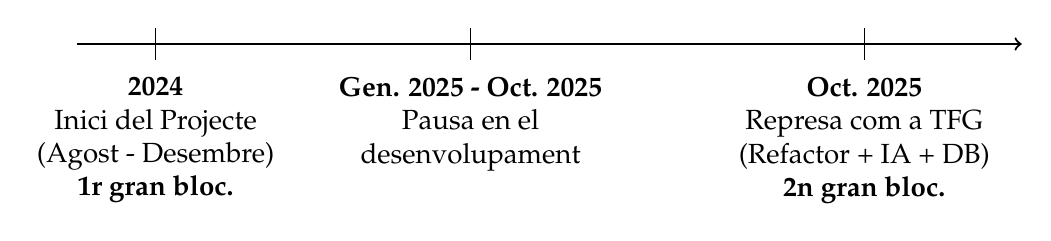
\begin{tikzpicture}
        % Draw the line
        \draw[thick, ->] (0,0) -- (12,0);
        
        % 2022 Node
        \draw (1,0.2) -- (1,-0.2);
        \node[align=center, below] at (1,-0.3) {\textbf{2024} \\ Inici del Projecte \\ (Agost - Desembre) \\ \textbf{1r gran bloc.}};
        
        % 2023 Node
        \draw (5,0.2) -- (5,-0.2);
        \node[align=center, below] at (5,-0.3) {\textbf{Gen. 2025 - Oct. 2025} \\ Pausa en el \\ desenvolupament};

        % Oct 2025 Node
        \draw (10,0.2) -- (10,-0.2);
        \node[align=center, below] at (10,-0.3) {\textbf{Oct. 2025} \\ Represa com a TFG \\ (Refactor + IA + DB) \\ \textbf{2n gran bloc.}};
    \end{tikzpicture}
    \caption{Línia temporal del desenvolupament del projecte NUMEN.}
    \label{fig:timeline}
\end{figure}

\subsection{Etapa 1: Naixement i Desenvolupament (2024)}
Aquesta primera etapa, compresa entre l'agost i el desembre de 2024, va néixer d'una forta motivació personal per ajudar a la meva mare, experta en numerologia, a automatitzar els complexos càlculs manuals que requeria la seva feina.

En aquesta primera etapa es van haver de prendre les decisions més importants del projecte, com ara el disseny de l'aplicació, el llenguatge de programació i les tecnologies a utilitzar. El desenvolupament va ser \textbf{purament manual i autodidacta}, sense l'ús d'Intel·ligència Artificial generativa per al codi. Amb l'ajuda de la meva mare i la referència del llibre de Martine Coquatrix, es va assolir la comprensió dels càlculs necessaris per realitzar les cartes numerològiques, ideant algoritmes simples per dur a terme l'automatització d'aquest coneixement.
El resultat d'aquesta fase va ser una aplicació \textbf{completament funcional} a nivell de càlcul: el sistema ja era capaç de generar totes les cartes, mapes i gràfics necessaris. La robustesa del nucli matemàtic de NUMEN és fruit d'aquesta dedicació artesanal, on cada línia de codi va ser escrita i validada manualment, creant una base sòlida i lliure de ``caixes negres''.

Aquest esforç manual atorga un valor afegit al projecte: tot i que avui dia eines com la IA Generativa permetrien aixecar un prototip similar en qüestió de dies, la robustesa i el control absolut sobre la lògica del nucli de NUMEN són totes decisions preses per mi, amb tot el procés evolutiu i reflexiu que comporta, ajudant enormament en el meu procés evolutiu i aprenentatge com a enginyer informàtic.

\subsection{Etapa 2: Professionalització Acadèmica (TFG 2025)}
Amb la represa del projecte com a Treball Final de Grau l'octubre de 2025, l'objectiu va virar de la funcionalitat pura cap a la \textbf{professionalització i l'escalabilitat}. En aquesta fase s'han implementat canvis estructurals crítics per convertir una eina d'ús personal en un producte de programari robust:

\begin{itemize}
    \item \textbf{Infraestructura al Núvol:} Integració de \textbf{Google Firestore} com a base de dades per persistir els estudis i \textbf{Google Firebase Hosting} per al desplegament web global.
    \item \textbf{Refactorització de la Impressió (Native PDF):} S'ha realitzat un canvi tècnic fonamental en el mòdul d'exportació. A la primera etapa, els informes s'imprimien realitzant una "captura de pantalla" del que veia l'usuari, fet que limitava la qualitat. En aquesta etapa, s'ha reescrit el sistema utilitzant llibreries de generació de PDF natiu, codificant plantilles vectorials que repliquen el disseny fidelment però amb qualitat professional, independent de la resolució de la pantalla.
    \item \textbf{Funcionalitat ``Compartir'' (Link 24h):} S'ha desenvolupat un sistema per generar enllaços temporals d'accés als informes, permetent al professional compartir digitalment l'estudi amb el client final de manera segura durant 24 hores.
    \item \textbf{Disseny Responsive:} Refactorització de la interfície per garantir la usabilitat en dispositius mòbils i tauletes, adaptant els gràfics complexos a pantalles petites.
    \item \textbf{Integració d'IA (Gemini):} Finalment, s'ha connectat l'API de Gemini (model Flash) per a la interpretació. És important notar que la IA només s'utilitza per enriquir el resultat amb text natural; no intervé en els càlculs, mantenint la fiabilitat de l'etapa anterior.
\end{itemize}

\section{Metodologia de Treball}
S'ha seguit una adaptació personalitzada de metodologies àgils. Les metodologies àgils són un enfocament de gestió de projectes que prioritza l'entrega ràpida i contínua de valor mitjançant cicles de treball curts i iteratius, permetent una adaptació flexible als canvis i una millora constant del producte final. Típicament, aquests cicles (coneguts com a \textit{Sprints} en marcs com Scrum) tenen una durada d'entre una i quatre setmanes. Donat que l'equip de desenvolupament està format per una única persona, s'ha optat per un enfocament iteratiu i incremental:
\begin{enumerate}
    \item \textbf{Disseny Inicial:} Definició de l'arquitectura i model de dades.
    \item \textbf{Implementació per Prioritats:} Codificació dels mòduls més influents i crítics (motor de càlcul) abans d'abordar la interfície d'usuari o la generació d'informes.
    \item \textbf{Refactorització Contínua:} Revisió constant del codi per millorar-ne l'eficiència i la llegibilitat a mesura que s'adquirien nous coneixements.
\end{enumerate}

\section{Declaració d'Ús d'Intel·ligència Artificial}
D'acord amb la normativa acadèmica i els principis de transparència, es declara explícitament l'ús d'eines d'Intel·ligència Artificial Generativa en aquest Treball Final de Grau.

\begin{itemize}
    \item \textbf{Desenvolupament de Software:} El nucli de l'aplicació, l'arquitectura i la lògica de negoci han estat desenvolupats manualment des de l'any 2024. L'ús d'IA en el codi s'ha limitat recentment a tasques de suport puntual, com la generació de consultes complexes a la base de dades o l'optimització de funcions específiques de \textit{prompting}.
    \item \textbf{Redacció de la Memòria:} S'han utilitzat models de llenguatge (com Google Gemini) com a assistents de redacció per a la revisió d'estil, correcció ortogràfica i estructuració de continguts, amb l'objectiu d'assolir un nivell de professionalitat i formalitat acadèmica excel·lent.
    \item \textbf{Autoria:} Tot el contingut generat o suggerit per la IA ha estat revisat, validat i editat exhaustivament, mantenint la responsabilitat total sobre la veracitat i originalitat del treball presentat. L'IA ha servit com a eina d'amplificació de capacitats, no com a substitut de l'autoria intel·lectual.
\end{itemize}

%% !TEX root = ../main.tex

\chapter{Planificació}
\label{Chapter4}

\section{Estratègia de Planificació}
Per tal de gestionar la complexitat del projecte i assegurar el compliment dels objectius establerts, s'ha optat per dividir el desenvolupament en diferents Paquets de Treball (PT). Aquesta estratègia permet focalitzar els esforços en tasques concretes i mesurables, facilitant el seguiment del progrés i la detecció primerenca de possibles desviacions.

La metodologia de treball seguirà un enfocament iteratiu i incremental, especialment en les fases de desenvolupament i validació, permetent incorporar el feedback de manera contínua.

\section{Paquets de Treball}
% Translations for Gantt Chart
\languagealias{catalan}{Catalan}
\deftranslation[to=Catalan]{August}{Agost}
\deftranslation[to=Catalan]{September}{Setembre}
\deftranslation[to=Catalan]{October}{Octubre}
\deftranslation[to=Catalan]{November}{Novembre}
\deftranslation[to=Catalan]{December}{Desembre}
\deftranslation[to=Catalan]{January}{Gener}
\deftranslation[to=Catalan]{February}{Febrer}

A continuació es detallen els paquets de treball definits per al projecte \textbf{NUMEN}.

\begin{table}[H]
    \centering
    \begin{tabular}{|p{0.25\textwidth}|p{0.70\textwidth}|}
        \hline
        \rowcolor{gray!20} \textbf{Nom del paquet} & \textbf{PT1: GESTIÓ I DOCUMENTACIÓ} \\ \hline
        \textbf{Descripció} & Gestió integral del projecte, reunions de seguiment i redacció de la memòria. \\ \hline
        \textbf{Requisits/Tasques} & 
        \begin{itemize}[noitemsep,topsep=0pt,leftmargin=*]
            \item Planificació inicial i definició d'objectius.
            \item Reunions periòdiques amb la tutora.
            \item Redacció dels capítols de la memòria.
            \item Revisió i correcció de la documentació.
        \end{itemize} \\ \hline
        \textbf{Lliuraments} & Memòria del TFG, Actes de reunió. \\ \hline
        \textbf{Temps} & Transversal (Tot el projecte) \\ \hline
    \end{tabular}
    \caption{Paquet de treball: Gestió i Documentació}
    \label{tab:pt1}
\end{table}

\begin{table}[H]
    \centering
    \begin{tabular}{|p{0.25\textwidth}|p{0.70\textwidth}|}
        \hline
        \rowcolor{gray!20} \textbf{Nom del paquet} & \textbf{PT2: ANÀLISI I DISSENY} \\ \hline
        \textbf{Descripció} & Definició dels requisits del sistema i disseny de l'arquitectura i la interfície. \\ \hline
        \textbf{Requisits/Tasques} & 
        \begin{itemize}[noitemsep,topsep=0pt,leftmargin=*]
            \item Anàlisi de requisits funcionals i no funcionals.
            \item Estudi del mètode numerològic de Coquatrix.
            \item Disseny de la Base de Dades.
            \item Disseny de la Interfície d'Usuari (UI/UX).
        \end{itemize} \\ \hline
        \textbf{Lliuraments} & Diagrames UML, Mockups de la interfície, Esquema de la BD. \\ \hline
        \textbf{Temps} & 3 setmanes \\ \hline
    \end{tabular}
    \caption{Paquet de treball: Anàlisi i Disseny}
    \label{tab:pt2}
\end{table}

\begin{table}[H]
    \centering
    \begin{tabular}{|p{0.25\textwidth}|p{0.70\textwidth}|}
        \hline
        \rowcolor{gray!20} \textbf{Nom del paquet} & \textbf{PT3: NUCLI NUMEROLÒGIC} \\ \hline
        \textbf{Descripció} & Implementació dels algoritmes de càlcul segons el mètode de Coquatrix. \\ \hline
        \textbf{Requisits/Tasques} & 
        \begin{itemize}[noitemsep,topsep=0pt,leftmargin=*]
            \item Implementació de la conversió lletra-número (Gematria).
            \item Càlcul de l'Arbre de la Vida personalitzat.
            \item Implementació de càlculs de cicles i etapes de vida.
            \item Tests unitaris dels algoritmes matemàtics.
        \end{itemize} \\ \hline
        \textbf{Lliuraments} & Mòdul de càlcul numerològic funcional i testejat. \\ \hline
        \textbf{Temps} & 4 setmanes \\ \hline
    \end{tabular}
    \caption{Paquet de treball: Nucli Numerològic}
    \label{tab:pt3}
\end{table}

\begin{table}[H]
    \centering
    \begin{tabular}{|p{0.25\textwidth}|p{0.70\textwidth}|}
        \hline
        \rowcolor{gray!20} \textbf{Nom del paquet} & \textbf{PT4: DESENVOLUPAMENT DEL SISTEMA} \\ \hline
        \textbf{Descripció} & Construcció de l'aplicació completa, integrant Frontend, Backend i Base de Dades. \\ \hline
        \textbf{Requisits/Tasques} & 
        \begin{itemize}[noitemsep,topsep=0pt,leftmargin=*]
            \item Configuració de l'entorn i repositori.
            \item Desenvolupament de l'API Backend.
            \item Implementació del Frontend i visualització gràfica.
            \item Integració amb la Base de Dades.
        \end{itemize} \\ \hline
        \textbf{Lliuraments} & Codi font de l'aplicació, prototip funcional. \\ \hline
        \textbf{Temps} & 5 setmanes \\ \hline
    \end{tabular}
    \caption{Paquet de treball: Desenvolupament del Sistema}
    \label{tab:pt4}
\end{table}

\begin{table}[H]
    \centering
    \begin{tabular}{|p{0.25\textwidth}|p{0.70\textwidth}|}
        \hline
        \rowcolor{gray!20} \textbf{Nom del paquet} & \textbf{PT5: INTEL·LIGÈNCIA ARTIFICIAL} \\ \hline
        \textbf{Descripció} & Integració de serveis d'IA per a la interpretació de resultats. \\ \hline
        \textbf{Requisits/Tasques} & 
        \begin{itemize}[noitemsep,topsep=0pt,leftmargin=*]
            \item Disseny de \textit{prompts} per a la interpretació numerològica.
            \item Integració amb l'API d'OpenAI/Gemini.
            \item Emmagatzematge de respostes per a futur entrenament.
            \item Refinament de la qualitat de les respostes.
        \end{itemize} \\ \hline
        \textbf{Lliuraments} & Mòdul d'interpretació per IA integrat. \\ \hline
        \textbf{Temps} & 3 setmanes \\ \hline
    \end{tabular}
    \caption{Paquet de treball: Intel·ligència Artificial}
    \label{tab:pt5}
\end{table}

\begin{table}[H]
    \centering
    \begin{tabular}{|p{0.25\textwidth}|p{0.70\textwidth}|}
        \hline
        \rowcolor{gray!20} \textbf{Nom del paquet} & \textbf{PT6: VALIDACIÓ I PROVES} \\ \hline
        \textbf{Descripció} & Verificació del sistema amb casos reals i correcció d'errors. \\ \hline
        \textbf{Requisits/Tasques} & 
        \begin{itemize}[noitemsep,topsep=0pt,leftmargin=*]
            \item Proves d'integració i sistema.
            \item Validació manual amb la "client" experta (mare).
            \item Comparació de resultats automàtics vs manuals.
            \item Correcció de bugs i ajustos finals.
        \end{itemize} \\ \hline
        \textbf{Lliuraments} & Informe de proves, Versió final del programari. \\ \hline
        \textbf{Temps} & 2 setmanes \\ \hline
    \end{tabular}
    \caption{Paquet de treball: Validació i Proves}
    \label{tab:pt6}
\end{table}

\section{Planificació Temporal}
El desenvolupament del projecte es divideix en dues fases temporals diferenciades. A continuació es mostren els cronogrames corresponents a la fase inicial (2024) i la fase de finalització com a TFG (2025-2026).

\begin{figure}[H]
    \centering
    \caption{Fase 1. 
    Desenvolupament Inicial (2024)}
    \label{fig:gantt_phase1}
    \makebox[\textwidth][c]{
    \begin{ganttchart}[
        vgrid={*6{draw=none}, *1{dotted}},
        hgrid,
        x unit=0.075cm,
        y unit chart=0.9cm,
        time slot format=isodate,
        time slot unit=day,
        calendar week text={\currentweek},
        bar/.append style={fill=udgblue!50},
        bar height=0.6,
        group right shift=0,
        group top shift=0.7,
        group height=.3,
        group peaks width={0.2},
        link/.style={->, thick}
    ]{2024-08-01}{2024-12-31}
        \gantttitlecalendar{year, month=name} \\
        
        % Phase 1
        \ganttgroup[name=p1_total]{Fase 1: Des.}{2024-08-01}{2024-12-31} \\
        \ganttbar[name=p1_analisi]{Anàlisi i Requisits}{2024-08-01}{2024-08-31} \\
        \ganttbar[name=p1_disseny]{Disseny}{2024-09-01}{2024-09-15} \\
        \ganttbar[name=p1_nucli]{Nucli i Algoritmes}{2024-09-15}{2024-11-30} \\
        \ganttbar[name=p1_front]{Frontend Inicial}{2024-11-01}{2024-12-31} \\
        
        \ganttlink{p1_analisi}{p1_disseny}
        \ganttlink{p1_disseny}{p1_nucli}
        \ganttlink{p1_nucli}{p1_front}
    \end{ganttchart}
    }
\end{figure}

\begin{figure}[H]
    \centering
    \caption{Fase 2: Finalització TFG (2025-2026)}
    \label{fig:gantt_phase2}
    \makebox[\textwidth][c]{
    \begin{ganttchart}[
        vgrid={*6{draw=none}, *1{dotted}},
        hgrid,
        x unit=0.075cm,
        y unit chart=0.9cm,
        time slot format=isodate,
        time slot unit=day,
        calendar week text={\currentweek},
        bar/.append style={fill=udgblue!50},
        bar height=0.6,
        group right shift=0,
        group top shift=0.7,
        group height=.3,
        group peaks width={0.2},
        link/.style={->, thick}
    ]{2025-09-01}{2026-01-31}
        \gantttitlecalendar{year, month=name} \\
        
        % Phase 2
        \ganttgroup[name=p2_total]{Fase 2: TFG}{2025-09-01}{2026-01-31} \\
        \ganttbar[name=p2_gestio]{Gestió i Memòria}{2025-09-01}{2026-01-20} \\
        \ganttbar[name=p2_refactor]{Refactorització i BD}{2025-09-15}{2025-10-31} \\
        \ganttbar[name=p2_ia]{Integració IA}{2025-11-01}{2025-11-30} \\
        \ganttbar[name=p2_validacio]{Validació i Proves}{2025-12-01}{2025-12-20} \\
        
        \ganttlink{p2_refactor}{p2_ia}
        \ganttlink{p2_ia}{p2_validacio}
    \end{ganttchart}
    }
\end{figure}
 
%% !TEX root = ../main.tex

\chapter{Marc de treball i conceptes previs}
\label{Chapter5}

\section{Entorn de Treball}

L'entorn de desenvolupament s'ha configurat per maximitzar la productivitat i la integritat del codi en un context de treball individual. Les eines principals utilitzades han estat:

\begin{itemize}
    \item \textbf{Sistema Operatiu:} Desenvolupament realitzat principalment sobre Windows.
    \item \textbf{IDE:} Visual Studio Code com a entorn de desenvolupament principal, equipat amb extensions per a Dart/Flutter i control de versions.
    \item \textbf{Control de Versions:} Ús de Git per a la gestió local del codi i GitHub com a repositori remot, seguint un flux de treball basat en \textit{main} i branques per funcionalitat.
    \item \textbf{Framework:} Flutter SDK (llenguatge Dart) per a la creació de l'aplicació multiplataforma.
    \item \textbf{Serveis al Núvol:} Gestió centralitzada mitjançant la consola de Firebase (Firestore, Hosting).
\end{itemize}

\section{Conceptes Previs: La Numerologia com a Domini}

Per comprendre la lògica de negoci implementada en \textbf{NUMEN}, és imprescindible definir els conceptes fonamentals de la numerologia segons el mètode de Martine Coquatrix. Des d'una perspectiva tècnica, podem considerar la numerologia com un sistema determinista de processament de dades, on les entrades (data de naixement i nom complet) es transformen mitjançant algoritmes específics en un conjunt de mètriques significatives.

A continuació es detallen els algoritmes i estructures de dades principals que conformen el nucli matemàtic de l'aplicació. Per a una descripció exhaustiva dels fonaments teòrics, la història de la numerologia i el significat detallat de cada número, consulteu l'\textbf{Annex \ref{AppendixA}}.

\subsection{Gematria i Conversió Alfanumèrica}
La base de tot càlcul numerològic textual és la conversió de lletres a valors numèrics. El sistema utilitzat assigna a cada lletra de l'alfabet llatí un valor de l'1 al 9, seguint un patró seqüencial.

La taula de conversió implementada és la següent:

\begin{table}[H]
    \centering
    \begin{tabular}{|c|c|c|c|c|c|c|c|c|}
        \hline
        \textbf{1} & \textbf{2} & \textbf{3} & \textbf{4} & \textbf{5} & \textbf{6} & \textbf{7} & \textbf{8} & \textbf{9} \\ \hline
        A & B & C & D & E & F & G & H & I \\ \hline
        J & K & L & M & N, Ñ & O & P & Q & R \\ \hline
        S & T & U & V & W & X & Y & Z &   \\ \hline
    \end{tabular}
    \caption{Taula de conversió Gematria (Sistema Pitagòric)}
    \label{tab:gematria}
\end{table}

És important destacar que caràcters com la `Ñ' s'assignen al valor 5 (igual que la `N'), i els accents o diacrítics s'ignoren (per exemple, `À' es tracta com `A').

\subsection{Reducció Teosòfica i Nombres Mestres}
La majoria de càlculs requereixen reduir qualsevol xifra superior a 9 a un sol dígit (de l'1 al 9). Aquest procés, conegut com a reducció teosòfica, consisteix a sumar els dígits del nombre de manera iterativa fins a obtenir-ne un d'elemental.

Matemàticament, per a un nombre $n$:
\[
R(n) = 
\begin{cases} 
n & \text{si } n \leq 9 \\
R(\sum_{d \in digits(n)} d) & \text{si } n > 9
\end{cases}
\]

\textbf{Excepció: Els Nombres Mestres}. Existeixen nombres especials que no s'han de reduir en determinats contextos: \textbf{11, 22 i 33}. Aquests es consideren ``Nombres Mestres'' i tenen una vibració superior. L'algoritme de reducció ha de contemplar aquesta excepció, verificant si el nombre resultant és mestre abans de continuar reduint.

\subsection{El Camí de Vida (Life Path)}
El Camí de Vida és una de les mètriques més rellevants, calculada a partir de la data de naixement. Representa la lliçó principal que l'individu ha vingut a aprendre.

L'algoritme de càlcul és el següent:
1. Es descompon la data en Dia, Mes i Any.
2. Es redueix cada component a un dígit (o nombre mestre).
3. Es sumen els tres components reduïts.
4. El resultat final es redueix novament si és necessari.

\subsection{La Inclusió (The Inclusion)}
La Inclusió és una eina complexa d'autoconeixement que analitza la distribució de les lletres del nom complet en nou àrees o ``cases''. Tècnicament, es tracta d'un histograma de freqüències on cada ``casa'' (de l'1 al 9) comptabilitza quantes vegades apareixen les lletres amb aquell valor numèric en el nom de la persona.

Aquest recompte genera el mapa d'\textbf{Habitants}:
\[ Habitants[i] = \text{count}(lletres \text{ amb valor } i) \quad \forall i \in [1,9] \]

A partir d'aquesta estructura base, es deriven altres vectors de dades mitjançant operacions matricials i lògiques:
\begin{itemize}
    \item \textbf{Matisos:} Relacionen els habitants entre si de manera recursiva.
    \item \textbf{Ponts:} Calculats com la diferència absoluta entre el valor de la casa i el seu habitant: $|Habitant[i] - (i+1)|$.
    \item \textbf{Evolució:} Indica cap a on tendeix l'energia de la casa.
    \item \textbf{Inconscient:} Revela patrons ocults basats en la posició de les lletres.
\end{itemize}

\subsection{Algorísmica del Nucli}
El cor de l'aplicació resideix en una sèrie d'algoritmes deterministes que transformen les dades d'entrada en mètriques significatives. A continuació, es detalla la lògica de negoci implementada per als càlculs més complexos.

\subsubsection{Càlculs Derivats del Nom}
A partir de la conversió gemàtrica, es calculen tres pilars fonamentals mitjançant la segregació de caràcters segons la seva tipologia fonètica:
\begin{itemize}
    \item \textbf{Ànima (Soul):} S'obté sumant exclusivament el valor de les \textbf{vocals} del nom complet. Representa la motivació interna.
    \item \textbf{Personalitat:} S'obté sumant exclusivament el valor de les \textbf{consonants}. Representa la projecció externa.
    \item \textbf{Expressió:} És la suma dels valors totals (Ànima + Personalitat) o de totes les lletres.
\end{itemize}

\subsubsection{Càlculs Derivats de la Data}
La data de naixement es processa per extreure'n cicles temporals, utilitzant operacions aritmètiques bàsiques però amb significats oposats:
\begin{itemize}
    \item \textbf{Desafiaments (Challenges):} Es calculen mitjançant la \textbf{resta} (valor absolut) entre els dígits reduïts del dia, mes i any (ex: $|Dia - Mes|$). Representen obstacles a superar.
    \item \textbf{Realitzacions (Pinacles):} Es calculen mitjançant la \textbf{suma} dels mateixos components. Representen els moments àlgids o metes.
\end{itemize}

\subsubsection{Algoritme del Número Llindar (NL)}
Un dels càlculs més complexos implementats és el del Número Llindar, el qual no segueix una fórmula aritmètica directa sinó una \textbf{lògica de prioritats condicional}. L'algoritme avalua l'histograma d'Habitants (Inclusió) en el següent ordre estricte:

\begin{enumerate}
    \item \textbf{Prioritat Kàrmica:} Si hi ha ``cases buides'' (habitants = 0), el NL és la suma d'aquestes cases buides.
    \item \textbf{Prioritat Dominant (Sobresurt):} Si un número apareix molt més que la resta (el seu valor és superior al segon màxim + 2), aquest esdevé el NL.
    \item \textbf{Prioritat per Repetició:} Si hi ha un empat en els valors màxims (més de 3 vegades repetit el màxim), es calcula una suma ponderada d'aquests.
    \item \textbf{Default (No Sobresurt):} Si no es compleix cap anterior, el NL és la suma de les dues cases amb major nombre d'habitants.
\end{enumerate}

\subsubsection{Càlcul d'Herències}
Les herències es calculen analitzant patrons específics en la distribució de la Inclusió, concretament observant la càrrega de les cases 1 (lideratge/pare) i 6 (família/responsabilitat), i com aquestes interactuen amb el total de lletres del nom.

\subsection{Algoritme de Visualització Dinàmica}
Una de les innovacions del sistema és la generació dinàmica de la figura representativa (l'home de Vitruvi) mitjançant la manipulació directa de vectors SVG.

\subsubsection{Lògica de Mapeig Vectorial}
La figura es descompon en regions (Cap, Braços, Cames, Tronc), i cadascuna està vinculada a coordenades numerològiques specífiques. L'algoritme recorre el mapa d'Habitants i la Data de Naixement i, per a cada coincidència, ``activa'' la regió corresponent del gràfic.

\subsubsection{Intensitat Cromàtica (Heatmap)}
No només es pinta la zona, sinó que es determina el color i la seva intensitat basant-se en la \textbf{freqüència d'aparició} del número:
\begin{itemize}
    \item \textbf{Escala de Vermells (Yang):} Utilitzada quan la coincidència prové directament dels dígits de la data de naixement (Dia, Mes, Any). A major repetició del dígit, més fosc i intens és el vermell (de \textit{LightSalmon} a \textit{DarkRed}).
    \item \textbf{Escala de Blaus (Yin):} Utilitzada quan la coincidència prové dels valors derivats de la Inclusió. Similarment, la intensitat del blau augmenta amb la freqüència (de \textit{PowderBlue} a \textit{Navy}).
\end{itemize}
Aquesta tècnica permet generar una representació visual única i immediata de l'energia del subjecte, on les zones fosques indiquen punts de màxima concentració energètica.

Aquests conceptes constitueixen la base teòrica sobre la qual s'ha construït el motor de càlcul de NUMEN.
 


%----------------------------------------------------------------------------------------
% THESIS CONTENT - APPENDICES
%----------------------------------------------------------------------------------------
\appendix % Cue to tell LaTeX that the following "chapters" are Appendices

% Include the appendices of the thesis as separate files from the Appendices folder
% Uncomment the lines as you write the Appendices
% !TEX root = ../main.tex

\chapter{Fonaments Teòrics de la Numerologia}
\label{AppendixA}

Aquest annex recull els fonaments teòrics que sustenten el sistema \textbf{NUMEN}, basats en la recerca realitzada per l'autor en el seu Treball de Recerca (TDR) i en l'obra de Martine Coquatrix.

\section{Què és la Numerologia?}

La numerologia és un conjunt de creences o tradicions que pretén establir una relació oculta entre els números, els éssers vius i les forces físiques o espirituals. També és una pràctica endevinatòria a través dels números \cite{wikipedia_numerologia}.

El seu estudi va ser popular entre els primers matemàtics, però no se la considera ja disciplina matemàtica. La comunitat científica fa temps que va relegar la numerologia a la categoria de pseudociència o superstició \cite{wikipedia_pseudociencia}, igual que l'astrologia pel que fa a l'astronomia, o l'alquímia, encara que aquesta última va tenir caràcter de protociència pel que fa a la química.

En numerologia, es diu que els números són un dels conceptes humans més perfectes i elevats. Segons els que la practiquen, la numerologia és la disciplina que pretén investigar la «vibració secreta» d'aquest codi i ensenyen a utilitzar els números en el seu benefici, per mitjà de l'estudi de la seva influència sobre persones, animals, coses i esdeveniments \cite{gonzalez_numerologia}.

L'any 530 a.C., Pitàgores, filòsof grec, va desenvolupar en forma metòdica una relació entre els planetes i la seva «vibració numèrica». Li va dir «la música de les esferes». Mitjançant el seu mètode de numerologia va afirmar que les paraules tenen un so que vibra en consonància amb la freqüència dels números com una faceta més de l'harmonia de l'univers i les lleis de la natura \cite{origen_numerologia}.

Com va dir Nikola Tesla: \textit{``Si vols conèixer els secrets de l'Univers, pensa en termes d'energia, freqüència i vibració''}. La física quàntica ha demostrat que som pura energia i informació vibrant a una determinada freqüència, i la numerologia estudia precisament la vibració dels números. Ens ensenya a sentir els números com una vibració.

\subsection{Origen de la Numerologia}
Encara que és difícil posicionar el seu origen amb precisió, avui podem identificar tres fonts o tres branques prominents:
\begin{itemize}
    \item \textbf{Numerologia Pitagòrica:} Pitàgores (500 aC) va ser qui va expandir aquest coneixement, fundant grups on s'estudiava el simbolisme dels números i la seva relació amb les lletres. Veia en pautes numèriques l'explicació dels fenòmens naturals i universals.
    \item \textbf{Simbolisme Cabalista:} Basat en la tradició mística jueva i l'Arbre de la Vida.
    \item \textbf{Simbolisme Cristià-Medieval:} Interpretació numèrica dels textos sagrats.
\end{itemize}

\section{L'Arbre de la Vida (Càbala)}

Per qualsevol qui defensi la numerologia, ``tot és número''. Els números representen l'armadura de l'univers, la seva defensa, el seu origen, la seva creació. L'Arbre de la Vida és un dels símbols cabalístics més importants del judaisme. Està compost per 10 esferes (sefirot) i 22 senders, cadascun dels quals representa un estat (sefira) que acosta a la comprensió de Déu i a la manera com ell va crear el món. La Càbala va desenvolupar aquest concepte com un model realista que representa un «mapa» de la Creació. Es considera la cosmologia de la Càbala \cite{wikipedia_arbol_vida}.

Alguns creuen que aquest «Arbre de la Vida» de la Càbala correspon a l'Arbre de la Vida esmentat a la Bíblia (Gènesi 2, 9) \cite{coquatrix_numerologia}.

\begin{figure}[H]
    \centering
    \includegraphics[width=0.4\textwidth]{Imatges/arbre_vida.png}
    \caption{Representació de l'Arbre de la Vida i els Sephiroth.}
    \label{fig:arbre_vida_tdr}
\end{figure}

Déu, en un estat de descans, decideix crear el món i projectar la seva força i la seva llum. Per fer-ho, ha d'imposar límits, passant de l'energia immensa de l'infinit a una energia definida. Així doncs, va formar aquest arbre de la vida compost per deu \textit{sephiroth} (recipients) que expressen deu essències o arquetips divins.

\subsection{Els Deu Sephiroth}
Cada sefira posseeix un nom que es pot comparar amb la seva ànima, i està associada a una jerarquia angèlica i a un planeta:

\begin{enumerate}
    \item \textbf{Kether (La Corona):} La voluntat primera. (Neptú / Serafins)
    \item \textbf{Hochmah (La Saviesa Revelada):} L'impuls dinàmic. (Urà / Querubins)
    \item \textbf{Binah (La Intel·ligència Concreta):} La forma que limita. (Saturn / Trons)
    \item \textbf{Hesed (La Misericòrdia i Abundància):} L'expansió. (Júpiter / Dominacions)
    \item \textbf{Geburah (El Rigor i la Força):} El límit i la disciplina. (Mart / Potències)
    \item \textbf{Tiferet (La Bellesa):} L'equilibri i l'harmonia. (Sol / Virtuts)
    \item \textbf{Netzah (La Victòria):} Les emocions i la natura. (Venus / Principats)
    \item \textbf{Hod (La Glòria):} L'intel·lecte i la comunicació. (Mercuri / Arcàngels)
    \item \textbf{Yesod (El Fonament):} L'inconscient i la memòria. (Lluna / Àngels)
    \item \textbf{Malkuth (El Regne):} El món físic i la realitat material. (Terra / Homes Perfectes)
\end{enumerate}

\textbf{Daat (El Coneixement):} És l'onzena sefira, misteriosa, la seu del coneixement. És el sol invisible, col·locat sobre el pilar central entre Kether i Tiferet. És el lloc de l'ànima.

En la part superior de l'Arbre de la Vida, per sobre de Kether, existeix un món infinit. Dintre d'aquest món, es troben diversos nivells d'existència negativa, que corresponen al 0; El Res i el Tot Possible:
\begin{itemize}
    \item \textbf{Ain Soph Aur:} Llum infinita.
    \item \textbf{Ain Soph:} Infinit, sense fi.
    \item \textbf{Ain:} Res, el punt més elevat.
\end{itemize}

Aquests tres nivells representen allò que transcendeix l'existència, la zona entre la Divinitat i la Creació. És l'absolut, el \textbf{NÚMERO DIVÍ PRIMORDIAL}, que ho conté tot i ho genera tot.

En aquesta existència negativa s'origina Kether, i a partir d'aquesta sefira, s'entra en la creació de l'univers. És com un flux d'energia divina que passa de sefira en sefira: de Kether passa per Hochmah, Binah, Hesed, Daat, Geburah, Tiferet, Netzah, Hod i finalment a Yesod, per acabar desembocant en Malkuth. En cada etapa, aquesta energia divina canvia de polaritat i d'aspecte. És com un riu que neix de Kether com una deu poderosa i cristal·lina que, mentre baixa per les diferents sefires, es va carregant de matèria i energia per acabar desembocant al mar, creant així EL MÓN \cite[p.~17]{coquatrix_numerologia}.


\subsection{Els Quatre Mons}
Segons la Càbala, l'Arbre es divideix en quatre mons:
\begin{itemize}
    \item \textbf{Azilout (Emanació):} Món dels arquetips (Kether). L'arrel dels mons.
    \item \textbf{Briah (Creació):} Món de l'esperit (Hochmah, Binah). Separació d'energies.
    \item \textbf{Yetzirah (Formació):} Món de la psique (Hesed a Yesod). Construcció i plasmació.
    \item \textbf{Assiah (Acció):} Món físic (Malkuth). On tenen forma els elements.
\end{itemize}

\subsection{El Cos Humà i l'Arbre}
El nostre cos està fet a imatge de l'Arbre de la Vida. De fet, portem a dintre de nosaltres l'esquema d'aquest arbre.
La columna vertebral correspon al pilar de l'equilibri, vinculant Kether amb Malkuth, la Corona amb el Regne, el cap amb els peus. Els dos costats del cos corresponen als dos pilars laterals, la Misericòrdia i el Rigor. En els tres pilars es recolzen els tres triangles ja esmentats. El triangle superior correspon al cap, la part del nostre cos oberta cap a l'infinit a través del xacra de la Corona. La Corona simbolitza la connexió de l'home amb el diví.
El cap té forma d'ou i representa allò que ha de néixer a la vida divina. En la iconografia hindú, el chakra Corona està representat per la flor de lotus de mil pètals que es desenvolupa al cim del crani. És per Kether per on el món diví baixa en l'home, el món de dalt, el «Mi», troba el món de baix, el «Ma» (Annick de Souzenelle). El segon triangle, format per Hochmah, Binah, Tiferet, està orientat cap avall i correspon a la regió cardíac-pulmonar. Aquí és on habita l'ésser espiritual, matriu de l'ésser diví, la nostra ànima. Entre el cap i el complex cardíac-pulmonar es troba el coll, comunicació entre l'ànima i l'obertura al diví. Quan Déu parla del seu «poble de la nuca rígida», li revela la ruptura de comunicació entre el cor i el cap, entre l'home i Déu. El tercer triangle invertit, que conté Netzah, Hod i Yesod, correspon al complex urogenital. Si es nodreix del món diví, l'home podrà obrir-se lentament a l'ésser espiritual que viu en ell. Si es nodreix només del món de baix i no es vincula amb l'ésser diví en ell mateix, coneixerà la mort: la matriu no haurà fructificat. La progressió en l'arbre es pot fer per diferents etapes. La primera etapa va de Malkuth fins al camí que uneix Hod a Netzah, és a dir, des dels peus fins als malucs i els ronyons. Correspon a les vèrtebres sacro-lumbars. En el desenvolupament de l'ésser correspon a la primera etapa, que és el naixement de l'ésser físic i l'etapa del «tenir». La segona etapa està continguda en el quadrilàter constituït per Hod, Netzah, Geburah i Hesed. Correspon al tronc, és a dir, a la part entre els malucs i les espatlles. És l'etapa de l'edat adulta. Correspon a les vèrtebres dorsals i al naixement de l'ésser espiritual. Quan l'home accedeix a aquesta etapa es troba en l'etapa de l'ésser. Es defineix aquesta etapa com el temps de pausa, de prova. Està formada pels quatre pilars, el 4 implica una noció d'estabilitat, de construcció sòlida, maduració i responsabilitat.
\section{Descripció i Simbolisme dels Números}

\begin{figure}[H]
    \centering
    \includegraphics[width=0.4\textwidth]{Imatges/numeros_tdr.png}
    \caption{Representació gràfica dels números.}
    \label{fig:numeros_tdr}
\end{figure}

\subsection{Yang i Yin}
\begin{itemize}
    \item \textbf{Yang (1, 3, 5, 7, 9):} Energia masculina, elements Foc i Aire. Són actius, analítics, racionals i competitius. Els agrada destacar i estar a primera fila.
    \item \textbf{Yin (2, 4, 6, 8):} Energia femenina, elements Aigua i Terra. Són intuïtius, flexibles, pacífics i col·laboradors. Privilegien la vida interior.
\end{itemize}

\subsection{Simbolisme Detallat}

\subsubsection{El Zero (0)}
El zero, és pot comparar amb un cercle que progressa fora del espai i el temps. És un vuit, que posseeix tot el potencial per ser omplert. Té un poder immens. Pot ser el tot i el no res. Com un ou, d'on neixen tots els altres números. Un número enigmàtic, considerat com a especial \cite{coquatrix_numerologia}.

En la reducció de la numerologia, és a dir, en la realització dels treballs numerològics, el zero no apareix, però potència el número resultant. PER EXEMPLE: 10 = 1 + 0 = 1. Però aquest 1, que prové del 10, és més potent.

\subsubsection{El Número 1}
És la representació de la unitat, l'origen del tot. La manifestació d'una força nova. Representa l'arquetip del \textbf{PARE}, referència psicològica molt important. És el pioner i el líder que obra els camins, que es llença amb decisió i autoritat als seus projectes. Injecta noves energies a les idees, i llença nous projectes intel·lectuals i mentals. Sempre vol ser el primer, i ser reconegut com el millor \cite{dela_numero_1}.

\begin{itemize}
    \item \textbf{COS HUMÀ:} Correspon a l'hemisferi cerebral esquerra, que determina el costat dret del nostre cos. És el centre de la voluntat, del potencial intel·lectual i abstracte, del pensament lògic, de l'acció.
    \item \textbf{TRAMPES DEL SEU EXCÉS:} Orgullós, dominador, egoista, ambiciós, impacient, irritable, tirànic, inflexible, intolerant, exigent, implacable, insensible.
\end{itemize}

\subsubsection{El Número 2}
De la unitat de l'1, passem a la dualitat del 2. Representa el principi femení. El dos, neix de l'1, i forma amb ell un sistema binari. D'aquesta manera, tenim dos pols: El Yang i el Yin \cite{calcuworld_numero_2}.

La grafia d'aquest número, està composta per corbes i línies rectes, per la qual cosa, indica la seva adaptabilitat i flexibilitat. És caracteritza per tenir una actitud de disponibilitat, sempre atent per escoltar i ser flexible. El número 2, vol ser i sentir, lentament, descobrint la seva afectivitat i sentiments interiors profunds. Té com a objectiu, donar i rebre.

És el número de la feminitat i maternitat. Correspon a l'arquetip de mare. Vol estimar i ser estimat, envoltar-se d'amor, viure al nivell dels seus sentiments, de la seva tendresa. Té por a la soledat, i sempre està buscant la fusió amb algú altre. A més, sempre compte amb la capacitat d'adaptar-se i d'actuar amb molta intuïció i diplomàcia. A través de la seva delicadesa, de la seva virtut d'escoltar i de poder acollir, pot arribar a canviar el curs de les coses i les opinions dels altres. ÉS EL NÚMERO DE LA COL·LABORACIÓ.

Posseeix un gran potencial artístic gràcies a la seva sensibilitat i apertura al món de la imaginació i els somnis. No té confiança en si mateix, i necessita sempre la aprovació d'algú altre per poder creure amb ell mateix. Sol viure amb complexa d'inferioritat, a no ser que sigui reconegut per algú altre. És incapaç de suportar els conflictes, i per això prefereix callar i no expressar el que sent, per temor a ser rebutjat pels altres. S'empassa les seves emocions, fins al punt d'asfixiar-se i destruir-se.

\begin{itemize}
    \item \textbf{COS HUMÀ:} Correspon a l'hemisferi cerebral dret, el món de la imaginació, la sensibilitat i la intuïció. Aquest hemisferi, determina la part esquerra del nostre cos, la part femenina i receptiva. Està relacionada també amb els òrgans dobles del cos, és a dir, els pulmons, els ronyons...
    \item \textbf{TRAMPES DEL SEU EXCÉS:} Dubte, dualitat, complexa d'inferioritat, falta d'autoestima i autodestrucció, vulnerabilitat, descontrol de les emocions, dependència, rol de víctima i inseguretat.
\end{itemize}

\subsubsection{El Número 3}
El 3, és la unió de l'1 i el 2. És un número perfecte, perquè conté la força de l'1 (energia masculina), i la sensibilitat del 2 (energia femenina). Representa l'arquetip del nen, fruit de la unió del pare i la mare \cite{euroresidentes_numero_3}.

La seva grafia està composta per corbes sensuals, amb tres puntes obertes que reflecteixen l'intercanvi amb els altres:
\begin{itemize}
    \item En el cap: la comunicació verbal.
    \item En el cor: la comunicació sentimental i emocional.
    \item En el ventre: La comunicació corporal i el plaer.
\end{itemize}

\begin{figure}[H]
    \centering
    \includegraphics[width=0.4\textwidth]{Imatges/tres.png}
    \caption{Representació del número 3.}
    \label{fig:numero_3}
\end{figure}



Té l'art de comunicar-se i expressar-se a través de la seva veu, la seva paraula. Posseeix un do per ensenyar i transmetre el seus coneixements. En el pla artístic, pot emprendre qualsevol projecte, degut al seu talent, originalitat i el seu desenvolupat sentit estètic. Necessita estimar i ser estimat per TOTS. Li agrada complaure i destacar. Ser reconegut pel seu públic. La admiració dels altres és la seva força, però també pot convertir-se en la seva debilitat.

Quan no se sent estimat i acceptat pels altres, pot tancar-se en si mateix, sofrir molt i tornar-se amargat i frustrat. Necessita estar envoltat pels seus amics, dels seus germans, de la seva família. Del seu grup de comunicació per compartir i gaudir de la vida en companyia. Està molt pendent de la mirada dels altres, i la necessita per tenir confiança en si mateix. LA SEVA IMATGE SOCIAL ÉS PRIMORDIAL, i quan aquest aspecte és torna obsessiu, pot arribar a convertir-se en una persona superficial.

Té l'art de viure bé el present. L'AQUÍ I L'ARA. És molt generós, li agrada compartir, és molt alegre, optimista i espontani. Adora les festes i les reunions, i posseeix un gran sentit de l'humor. El seu públic li resulta tant indispensable, que pot passar la seva vida actuant en rols determinats, sense viure la seva pròpia identitat. Té dificultats per viure en soledat, ja que tem enfrontar-se a la seva pròpia veritat.

\begin{itemize}
    \item \textbf{TRAMPES DEL SEU EXCÉS:} Frivolitat, superficialitat, agitació, dispersió, falta d'identitat, irresponsabilitat, vanitat, inestabilitat.
\end{itemize}

\subsubsection{El Número 4}
El seu element és la terra, que la transforma a través del seu treball. És el número de la encarnació. La seva grafia és un conjunt de rectes, amb angles ben definits, que inspiren fermesa i seguretat. Una imatge que recorda al tro d'un rei \cite{celeste_numero_4}.

El seu símbol, és el quadrat o el cub. Ens inspira estabilitat, equilibri i força. L'arquetip del 4 són les arrels. Representa la base sobre la qual construïm la nostra vida. La seva força radica en les normes establertes. Abans de donar un pas, necessita saber cap a on va dirigit. Per aquesta raó, a vegades avança molt lentament i li falta flexibilitat. És molt fidel, i sempre necessita aferrar-se a les tradicions de la seva terra natal i de la seva família. Com a conseqüència, se sent responsable del patrimoni material familiar. És el número del treball i la organització. Li agrada el treball ben fet, i dedicarà tots els seus esforços per complir els seus deures. Ha de tenir en compte, però, a no omplir-se de càrregues extres.

\begin{itemize}
    \item \textbf{COS HUMÀ:} Representa la part dura del cos, és a dir, l'esquelet i les dents.
    \item \textbf{TRAMPES DEL SEU EXCÉS:} Bloqueig mental i emocional, melancolia, rigidesa, obsessió per l'ordre, tosquedat, materialisme, obsessió per el treball, avarícia, inflexibilitat, dogmatisme i poca flexibilitat mental.
\end{itemize}

\subsubsection{El Número 5}
S'ubica a mig camí entre l'1 i el 9. Té l'energia exterior de l'1, obrint camins i lluitant en busca de nous reptes, i l'energia interior del 9, per la seva necessitat de reflexió. Està associat a Mart, el Déu de la guerra. La seva imatge és la d'un rei energètic que va a la batalla a fi de conquistar altres regnes: VIURE INSEGURETATS I CÓRRER RISCOS \cite{celeste_numero_5}.

El seu símbol és el pentagrama, i la seva grafia consisteix en una barra horitzontal superior que representa el seu gran desenvolupament mental, la seva curiositat sense límits i la seva gran capacitat d'anàlisi. Aquesta barra, recolzada sobre una corba, representa l'energia vital i sexual. Per un número 5, el vital és sentir-se lliure de llaços innecessaris. Necessita galopar lliurement sense sentir-se empresonat sota convencionalismes i regles. És rebel amb el seu mode de pensar i viure. És conscient del poder de la seva energia, i ha d'aprendre a dominar-la i controlar-l. Així mateix, ha de mantenir fermes les rendes del seu cavall, amb molta disciplina i rigor, pel contrari, acabaria desbocat.

Sempre busca experiències noves pel pur plaer d'experimentar, però, encara que a vegades cremi les seves ales per volar massa a prop del sol, aquest sempre està llest per cobrar el preu dels seus errors. És molt honest, i sempre juga net. El número 5, ha de saber, que també té dificultats, doncs mai acaba els seus projectes personals, degut a que sempre s'impacienta i comença a interessar-se per altres projectes. Córrer el risc de convertir-se en un ``picaflor'', que va de flor en flor en busca del no res. Per aquesta raó, és essencial que s'escolti a si mateix i mediti les seves decisions. És una aventurer per naturalesa, i sempre està disposat a viure tot tipus d'aventures i reptes físics/intel·lectuals. Se sent permanentment atret pels viatges i els descobriments d'altres cultures, però sempre necessita tornar als seus inicis. Degut a això, té el do dels idiomes.

Aquesta força vital, el pot portar a excessos: hiperactivitat, consumisme cultural... pot caure al descontrol, abusar de l'alcohol i el tabac, les drogues, realitzar experiències perilloses... el seu temperament explosiu el porta a situacions de risc. Per això, és important que el número cinc realitzi esport, per calmar aquesta hiperactivitat i equilibrar la seva energia.

\begin{itemize}
    \item \textbf{COS HUMÀ:} Representa el mode de viure la nostre part masculina Yang i la nostre energia vital, canalitzada a través de l'energia sexual o creativa. Representa el KI, el nostre centre energètic.
    \item \textbf{TRAMPES DEL SEU EXCÉS:} Irritabilitat, violència, agressivitat, inconstància, llibertinatge, addiccions (sexe, alcohol, drogues...)
\end{itemize}

\subsubsection{El Número 6}
És el centre de l'amor. El 6, es representa amb dos triangles encastats que formen el segell de Salomó, l'estrella de sis puntes \cite{celeste_numero_6}.

La grafia del sis, és una única corba que s'embolcalla sobre si mateixa. La seva base rodona, representa un ventre, simbolisme de la fertilitat i de l'amor. Viu segons la seva sensibilitat i les seves emocions. És el número de la feminitat que aporta pau i harmonia. Ens convida al descans, a la flexibilitat i la apertura del cor. La seva prioritat i desig és donar, protegir i cuidar als altes. Per contra, li costa molt donar i rebre. Sovint arribar al sacrifici, oblidant-se de si mateix. Per evitar aquesta situació, el número sis ha d'amar-se i cuidar-se en primer lloc, per poder entregar un amor equilibrat i sa. Inclús, pot arribar a ser possessiu i manipular afectivament als altres, a fi d'aconseguir ser amat i amar. Pot arribar a tenir pànic ha ser abandonat pel seus éssers estimats.

Se sentirà satisfet en professons que estan relacionades amb el cos i la salut, com per exemple medicina, estètica, massatgista... A més, posseeix un gran poder creatiu, i és capaç d'apreciar la bellesa visible i invisible dels sers.

L'arquetip del sis, representa la forma de viure la nostre part femenina Yin. Degut a la seva gran sensibilitat és bastant vulnerable, i sol viure bastantes crisis d'identitat i desequilibris emocionals forts. A més, també pot caure en l'apatia i la comoditat, conformant-se i sen mandrós.

\begin{itemize}
    \item \textbf{COS HUMÀ:} Representa el plexe cardíac, el cor, el lloc de la nostre ànima. El centre de les emocions.
    \item \textbf{TRAMPES DEL SEU EXCÉS:} Vulnerabilitat, fragilitat, possessió, manipulació, gelós, sacrifici, frustració, culpabilitat, obsessió, depressió, apatia i mandra.
\end{itemize}

\subsubsection{El Número 7}
És el número de la espiritualitat. És l'enllaç entre l'humà i el diví. El número sagrat per excel·lència. Sol associar-se a la bellesa i a la perfecció, sovint també, a les victòries. El 7, ens introdueix en la bellesa espiritual, simbolitzada en el Sabbat (sèptim dia), quan Déu descansa per admirar la perfecció de la creació \cite{celeste_numero_7}.

El 7 ens convida a trobar la unitat interior després d'un llarg aprenentatge personal que requereix autocontrol, exigència i una profunda concentració.

La seva grafia s'assembla al número 1, però amb un cap més desenvolupat, més sobrecarregat que sembla inclinar-se degut al seu pes de saber i coneixement. La seva base es fràgil i poc estable.

Té un sentit de la bellesa i de l'estètica que l'impulsa a buscar permanentment l'elegància. És molt sensible a la naturalesa i necessita estar en contacte amb ella. Necessita saber i aprendre, recolzant-se en llibres, escrits o documents. Tota la seva vida està buscant coneixements. Degut a això, és molt savi. Avança amb constància per aconseguir donar respostes a les grans interrogacions i enigmes existencials, descobrint les grans veritats. És el número dels grans místics, teòlegs i filòsofs que ens permeten accedir a una realitat superior. L'excés del treball mental, però, pot ocasionar-li dificultats per viure les contingències materials i expressar els seus sentiments. És difícil per aquesta persona, connectar-se amb el seu cos i el seu cor.

Necessita la soledat i el silenci a l'hora de meditar, contemplar i reflexionar. No obstant, això pot desencadenar a tancar-se en la seva ``torre de marfil'', i aïllar-se dels altres. Pot arribar a viure amb massa serietat i austeritat. Aquest excés de saber, pot provocar en ell actituds d'orgull, superioritat, menyspreu i sarcasme.

Si no aconsegueix els seus ideals, pot caure en una depressió o procés d'autodestrucció aïllant-se per complet del món.

\begin{itemize}
    \item \textbf{COS HUMÀ:} El número 7, està relacionat amb l'hemisferi cerebral esquerra, el lloc de la voluntat, la lògica i l'anàlisi. Correspon al chakra del tercer ull, que ens permet l'apertura espiritual.
    \item \textbf{TRAMPES DEL SEU EXCÉS:} Intransigència, intolerància, sarcasme, supèrbia, soledat, aïllament, pessimisme, auto-càstig, depressió i desequilibri mental.
\end{itemize}

\subsubsection{El Número 8}
És la manifestació de la intel·ligència perfecta i la capacitat de transformar la matèria. Aquest caduceu, està compost per dos parts simètriques que ens ajuden a comprendre millor el simbolisme del número 8 \cite{euroresidentes_numero_8}:
\begin{itemize}
    \item La serpentina de l'esquerra, representa el que rebem de l'univers: talents i dons.
    \item La serpentina de la dreta correspon a la manera en que retornem a l'univers els fruits de la Terra transformada.
    \item La vara del centre simbolitza la mediació entre Déu i l'Home.
\end{itemize}

El 8 és el símbol del Kundalini, de l'energia sexual, de la creativitat que ens ajuda a entrar en altres nivells de consciència. Com es pot veure en la seva grafia, les energies circulen des de dalt fins a baix, com si fos un rellotge de sorra. Representa el símbol de l'infinit en posició vertical.

El 8, representa el nostre poder, el nostre talent. A més, el 8, per ser dos vegades 4, és sòlid, responsable i té un gran sentit del concret. Té una gran personalitat d'organització i realització. És un número que comparteix aspectes Yin i Yang. El seu aspecte Yin, l'ajuda a prendre's el seu temps, preparar estratègies i madurar els seus projectes abans de llançar-se a l'acció, mentre que el seu aspecte Yang, l'ajuda amb una gran capacitat d'organització, rendiment i producció.

Per ser reconegut pels altres, necessita afirmar el seu poder material i econòmic. No pot viure sense treballar. Li agraden els reptes, i els afronta amb coratge i audàcia. Es capaç de realitzar qualsevol projecte. Darrere aquesta aparença exigent i autoritària, és generós i bondadós quan se sent amat pels altres. A més, posseeix un gran sentit de la justícia i l'honestedat.

Aquesta aparença exterior de poder i seguretat, pot amagar una gran fragilitat interior. És un número tant fort i amb tanta energia, que fàcilment pot cometre excessos de poder, orgull i dominació.

\begin{itemize}
    \item \textbf{COS HUMÀ:} Representa el plexe solar, i tots els seus aspectes de potència i vulnerabilitat.
    \item \textbf{TRAMPES DEL SEU EXCÉS:} Orgull, materialisme, cobdícia, supèrbia, arrogància, tirania, despotisme, autoritarisme, agressivitat, violència, crueltat i impaciència.
\end{itemize}

\subsubsection{El Número 9}
El número 9 és l'apertura de la ment i l'esperit. És l'últim número d'una sola xifra, que ens proposa anar més enllà dels nostres límits, i obrir-nos camins cap a horitzons més amplis. Al tarot, és el símbol de l'ermità, el que viu i manté la seva llum interior. El número Maestre interior, que necessita la seva llibertat física i espiritual per transmetre la saviesa al món \cite{celeste_numero_9}.

La seva grafia és un 6 invertit, i tanmateix, com el 6, està format únicament per corbes que evoquen les relacions amb aspectes sensibles i receptius. La diferència entre el 6 i el 9, doncs, mentre el 6 viu els seus sentiments i les seves emocions, el 9 exposa totes les seves energies al seu cap. La seva debilitat, és tanmateix la seva virtut. És com un globus que està molt carregat d'idees, somnis... però que té una connexió fràgil i poc estable amb la terra.

Per ser 3 vegades 3, viu en el seu món imaginari, per la qual cosa, també posseeix un gran creativitat i sensibilitat artística molt aguda.

El número del coneixement i misticisme per la seva connexió directe entre el seu cor i l'energia còsmica. El número del visionari. Compte amb una compassió que li permet captar els missatges de patiment que emeten els altres, i sentir la necessitat d'ajudar-los. Un número altruista, amb una vocació humanitària; viu amb l'ideal d'ajudar als més dèbils. El número de la compassió i la tolerància.

És tant idealista, compassiu i generós, que pot arribar a l'abnegació, oblidant-se de si mateix, posicionant als altres com la seva única prioritat. A més, si no aconsegueix el seu objectiu d'ajudar als altres, pot arribar a caure en l'autodestrucció i depressió. El 9, té problemes per acceptar les regles i exigències de la vida quotidiana, perquè prefereix refugiar-se al seu món imaginari.

\begin{itemize}
    \item \textbf{COS HUMÀ:} Representa el chakra corona, i la connexió amb els mons superiors, degut a la seva descendència en Yesod.
    \item \textbf{TRAMPES DEL SEU EXCÉS:} Utopia, falta de connexió amb la realitat, inconsistència, aïllament, mandra, marginació, depressió, comportaments agressius, orgull, dominació i autodestrucció.
\end{itemize}

\subsection{Els Nombres Mestres (11, 22, 33)}
Són números compostos per deu xifres idèntiques. Tenen una energia especial que requereix grans esforços i disponibilitats per part de la persona que el viu. Aquests números mestres, acompanyes a l'evolució de la humanitat, i actualment poden viure l'11, el 22 i el 33 \cite{adivinario_numeros_maestros}.

Són regales o carismes que ens ofereix l'univers per construir-nos, créixer i posar-nos al servei de la comunitat.

Aquests números mestres, són la simplificació dels números de l'1 al 9. És a dir, són números amb una potència molt més elevada. Per exemple:
\begin{itemize}
    \item 11 = 1 + 1 = 2 $\rightarrow$ l'onze, reduït, és un 2, i és manifesta com a tal, quan aquest aconsegueix viure en harmonia els aspectes del 2. Quan aquest, aconsegueix llimar les dureses de les trampes del seu excés, quan aconsegueix viure en pau i felicitat amb si mateix.
    \item 22 = 2 + 2 = 4
    \item 33 = 3 + 3 = 6
\end{itemize}

Aquests números mestres, que representen vibracions molt elevades, és viuen en certs moments de la vida, en certs cicles o anys, propers a l'evolució del ser. Però, aquests necessiten estar sostinguts per números energèticament forts, com l'1, el 5 o el 8.

No són números fàcils de viure, per les seves potents vibracions, la persona els ha d'acceptar, i ser conscient de la seva energia, no caure en la superioritat. Són números que ens indiquen que tenim un potencial més elevat, per col·laborar amb l'evolució de la terra i ajudar als altres.

\subsubsection{EL NÚMERO 11: ``Missatger Diví''}
Està compost per dos vegades 1, per la qual cosa, necessita ser reconegut i afirmar-se amb autoritat. A la vegada, representa el dos (1+1=2), la saviesa de l'arbre de la vida. Per aquest motiu, se l'anomena el missatger diví.

S'assembla al número 9, però amb una missió més elevada. Apareix en busca d'una veritat profunda. Està dotat de força moral fora del comú, així com una intel·ligència subtil i un potent magnetisme intel·lectual.

Però aquest número pot tenir també els seus riscos i trampes, degut a la seva barreja de dos vegades 1, i del 2:
\begin{itemize}
    \item Vulnerabilitat emocional.
    \item Nervis i impaciència.
    \item Un camí de vida que ha de recórrer amb saviesa i evitant els excessos.
    \item Complexa de superioritat, excés d'autoritat o manipulació.
\end{itemize}

\subsubsection{EL NÚMERO 22: ``Constructor de Futurs''}
És presentat com un inventor apassionat, un visionari amb una gran sensibilitat, un organitzador genial. El seu objectiu és realitzar grans projectes, amb idees noves i futuristes. És el número de la superació per aconseguir propòsits més elevats. Però el 22 pot tenir també els seus límits:
\begin{itemize}
    \item La pèrdua de l'equilibri psicològic quan és deixa portar per corrents contradictòries.
    \item La mala gestió de les emocions. És el punt dèbil del 22. Pot viure tensions afectives i conflictes racionals.
    \item L'excés de tensions que prové d'una energia física mal distribuïda o mal utilitzada.
\end{itemize}

\subsubsection{EL NÚMERO 33: ``L'amor incondicional''}
Quan ens trobem amb un 33, és necessari veure si la persona és capaç de viure l'aspecte del 6 amb harmonia i equilibri. El 33 és el número del sacrifici, de l'amor perfecte, de la compassió i la comprensió.

El número dels grans mesters. Poques persones son capaces de viure'l amb equilibri perquè suposa un gran discerniment per evitar caure en l'excés de l'abnegació i sacrifici.

\section{La Inclusió}

La inclusió és un camí d'autoconeixement a través de nou cases, o nou aspectes de la vida. Cada casa estarà ocupada per un ``habitant'', que estarà en evolució constant. Aquests ``habitants'' transmeten els missatges qualitatius i ens indiquen de quina forma viurem aquests aspectes de la vida. Representen les eines de base que tenim al néixer.

\subsection{Com construir la Inclusió}

Hem d'assignar a cada lletra el seu valor, d'acord amb el quadre següent:

\begin{table}[H]
    \centering
    \begin{tabular}{|c|c|c|c|c|c|c|c|c|}
        \hline
        \textbf{1} & \textbf{2} & \textbf{3} & \textbf{4} & \textbf{5} & \textbf{6} & \textbf{7} & \textbf{8} & \textbf{9} \\
        \hline
        A & B & C & D & E & F & G & H & I \\
        J & K & L & M & N, Ñ & O & P & Q & R \\
        S & T & U & V & W & X & Y & Z & \\
        \hline
    \end{tabular}
    \caption{Taula de conversió lletra-número per a la Inclusió.}
    \label{tab:inclusio_lletres}
\end{table}

Per construir la inclusió, es compta quantes lletres hi ha de cada valor numèric en el nom complet (noms i cognoms).

EXEMPLE: 
\begin{itemize}
    \item \textbf{Nom:} DAVID
    \item \textbf{Cognom pare 1:} QUINTANILLA
    \item \textbf{Cognom mare 1:} JIMENEZ 
    \item \textbf{Cognom pare 2:} GARCIA
    \item \textbf{Cognom mare 2:} MOLINA
\end{itemize}

\begin{figure}[H]
    \centering
    \includegraphics[width=0.8\textwidth]{Imatges/exemple.png}
    \caption{Exemple de la inclusió amb el nom DAVID QUINTANILLA}
    \label{fig:numero_exemple}
\end{figure}

\subsection{Les 9 Cases o les Nou Àrees de la Vida}

\begin{itemize}
    \item \textbf{CASA 1:} L'estructura de l'ego, identitat en el món, dinàmica d'afirmació, relació amb el pare.
    \item \textbf{CASA 2:} La forma de viure les emocions, capacitat d'escoltar i acollir, relació amb la mare, feminitat.
    \item \textbf{CASA 3:} Relació amb els altres (germans, amics), creativitat, expressió personal, el nen interior.
    \item \textbf{CASA 4:} Món material, treball, cos físic, bases personals (història familiar), compromís.
    \item \textbf{CASA 5:} Adaptació al canvi, capacitat d'anàlisi, llibertat, energia vital i sexualitat.
    \item \textbf{CASA 6:} Relacions afectives, responsabilitat familiar, amor a un mateix, benestar, harmonia.
    \item \textbf{CASA 7:} Espiritualitat, reflexió, coneixement, esquemes mentals, herències culturals.
    \item \textbf{CASA 8:} Talents, estratègia, realització, poder material, estatus social.
    \item \textbf{CASA 9:} Consciència universal, saviesa interior, servei humanitari, inconscient.
\end{itemize}

\subsection{Els Habitants: Formes de matisar les Cases}

Els habitants ens permetran entendre com o de quina manera vivim cada aspecte del nostre ser, a través de les nou cases.

\begin{itemize}
    \item \textbf{HABITANT 1:} Autònoma, amb autoritat, innovadora. Risc: Impaciència, dominació, orgull.
    \item \textbf{HABITANT 2:} Sensible, tendre, diplomàtica. Risc: Dubte, inseguretat, pors afectives.
    \item \textbf{HABITANT 3:} Creativa, comunicativa, alegre. Risc: Superficialitat, dispersió, necessitat de reconeixement.
    \item \textbf{HABITANT 4:} Estructurada, responsable, pacient. Risc: Rigidesa, pors materials, excés de responsabilitat.
    \item \textbf{HABITANT 5:} Dinàmica, lliure, aventurera. Risc: Inestabilitat, agressivitat, dispersió.
    \item \textbf{HABITANT 6:} Harmoniosa, servicial, responsable. Risc: Possessivitat, sacrifici, culpabilitat.
    \item \textbf{HABITANT 7:} Reflexiva, profunda, perfeccionista. Risc: Intolerància, aïllament, supèrbia.
    \item \textbf{HABITANT 8:} Eficient, constructiva, estratègica. Risc: Dominació, materialisme, agressivitat.
    \item \textbf{HABITANT 9:} Intuïtiva, idealista, compassiva. Risc: Desconnexió de la realitat, frustració, utopia.
\end{itemize}

%\include{Appendices/AppendixB}
%\chapter{Manual del Desenvolupador}
\label{appendix:manual_desenvolupador}

Aquest annex serveix com a guia tècnica detallada per a configurar l'entorn de desenvolupament local, permetent a futurs col·laboradors executar, depurar i desplegar el projecte NUMEN.

\section{Preparació de l'Entorn}

Abans de clonar el repositori, cal assegurar-se que la màquina de desenvolupament compleix amb els requisits previs.

\subsection{Instal·lació de Flutter SDK}
El projecte es basa en el framework Flutter. Cal descarregar la versió estable més recent des del lloc oficial (\url{https://flutter.dev}) i afegir el binari al \texttt{PATH} del sistema.

\begin{lstlisting}[language=bash, caption={Verificació de la instal·lació de Flutter}]
flutter doctor
\end{lstlisting}

\subsection{Node.js i NPM}
Les eines de línia de comandes de Firebase (\texttt{firebase-tools}) depenen de Node.js. Cal instal·lar la versió LTS de Node.js, que inclou el gestor de paquets NPM.

\begin{lstlisting}[language=bash, caption={Instal·lació de Firebase CLI via NPM}]
npm install -g firebase-tools
firebase login
\end{lstlisting}

\subsection{Visual Studio Code i Extensions}
L'entorn recomanat (IDE) és Visual Studio Code (VS Code). Per a una experiència òptima amb Flutter, es recomana instal·lar les extensions oficials:
\begin{itemize}
    \item \textbf{Flutter} (Dart-Code.flutter)
    \item \textbf{Dart} (Dart-Code.dart-code)
\end{itemize}

\section{Configuració Inicial del Projecte}

Un cop clonat el repositori, cal instal·lar les dependències i configurar els serveis del núvol.

\subsection{Instal·lació de Dependències}
Des de l'arrel del projecte, executar:
\begin{lstlisting}[language=bash]
flutter pub get
\end{lstlisting}

\subsection{Configuració de Firebase (FlutterFire)}
Per vincular el projecte local amb el projecte de Firebase al núvol, s'utilitza l'eina \texttt{flutterfire\_cli}. Si és el primer cop que es configura en una màquina nova:

\begin{lstlisting}[language=bash, caption={Activació i configuració de FlutterFire}]
dart pub global activate flutterfire_cli
flutterfire configure
\end{lstlisting}

Aquesta comanda guiarà a l'usuari per seleccionar el projecte de Firebase existent i generarà automàticament el fitxer \texttt{lib/firebase\_options.dart} amb les credencials actualitzades per a cada plataforma (Web, Android, iOS, Windows).

\section{Depuració i Execució}

Per facilitar la depuració en VS Code, el projecte inclou una configuració de llançament predefinida. No obstant això, donat que es requereix la injecció de la clau d'API, es recomana configurar el fitxer \texttt{.vscode/launch.json} o utilitzar arguments.

\subsection{Configuració de launch.json}
Es recomana configurar el fitxer \texttt{.vscode/launch.json} per utilitzar el paràmetre \texttt{--dart-define-from-file=.env}. Això permet que VS Code llegeixi automàticament totes les variables del fitxer d'entorn sense haver de llistar-les manualment.

\begin{lstlisting}[caption={Exemple de configuració launch.json optimitzada}]
{
    "version": "0.2.0",
    "configurations": [
        {
            "name": "numerologia_flutter (Web)",
            "request": "launch",
            "type": "dart",
            "args": [ "-d", "chrome" ],
            "toolArgs": [
                "--dart-define-from-file=.env"
            ]
        }
    ]
}
\end{lstlisting}

Amb aquesta configuració, el desenvolupador pot senzillament prémer la tecla \textbf{F5} (o fer clic a "Start Debugging") per compilar i executar l'aplicació amb totes les claus configurades correctament, agilitzant significativament el cicle de desenvolupament.

\section{Automatització del Desplegament}

Tal com s'ha descrit al Capítol \ref{chapter:implantacio_resultats}, el desplegament a producció està automatitzat mitjançant l'script \texttt{tools/deploy\_prod.bat}. Aquest script requereix un fitxer \texttt{.env} a l'arrel del projecte amb la clau d'API vàlida.

\begin{lstlisting}[language=bash, caption={Execució del desplegament}]
./tools/deploy_prod.bat
\end{lstlisting}

Aquest procés netejarà l'entorn, compilarà l'aplicació en mode \emph{release} (injectant la clau des del \texttt{.env}) i la pujarà a Firebase Hosting.


\section{Guia d'Instal·lació i Codi PWA}
\label{sec:pwa_guide}

L'aplicació NUMEN és una \textit{Progressive Web App} (PWA), el que permet instal·lar-la com si fos una aplicació nativa sense passar per les botigues d'aplicacions (App Store / Play Store). El comportament d'instal·lació varia segons el dispositiu.

\subsection{Escriptori (Windows / macOS)}
En navegadors basats en Chromium (Google Chrome, Microsoft Edge, Brave), el navegador detecta automàticament que el lloc web és una PWA.
L'usuari veurà una icona d'instal·lació a la part dreta de la barra de direccions (veure Figura \ref{fig:pwa_desktop}).

\begin{figure}[H]
    \centering
    \includegraphics[width=0.6\textwidth, frame]{Imatges/pwa_desktop_install.png}
    \caption{Icona d'instal·lació PWA a la barra de direccions (Google Chrome).}
    \label{fig:pwa_desktop}
\end{figure}

També és possible instal·lar l'aplicació des del menú d'opcions del navegador (els tres punts verticals $\vdots$) seleccionant ``Instal·lar NUMEN'' o ``Afegir a la pantalla d'inici''.

\subsection{Dispositius iOS (iPhone / iPad)}
A diferència d'Android o Windows, l'ecosistema d'Apple (iOS) no mostra cap avís automàtic per instal·lar aplicacions web. Això representa una barrera d'entrada per a l'usuari final.

Per solucionar-ho, s'ha implementat un component visual personalitzat (\texttt{pwa\_install\_prompt.dart}) que detecta si l'usuari navega des d'un iPhone (mitjançant \textit{User Agent}) i si l'app no està encara en mode pantalla completa (\textit{standalone}).
Si es compleixen aquestes condicions, es mostra un quadre de diàleg explicatiu amb els passos manuals a seguir:

\begin{enumerate}
    \item Prémer el botó \textbf{Compartir} de Safari (icona quadrada amb fletxa cap amunt).
    \item Seleccionar l'opció \textbf{``Afegir a l'inici''} (\textit{Add to Home Screen}).
\end{enumerate}

\subsection{Codi Font: Detecció i Prompt iOS}
A continuació es mostra el codi Dart encarregat de la detecció del navegador i la renderització del prompt d'ajuda per a usuaris d'iOS.

\begin{lstlisting}[language=Dart, caption={Lògica de detecció i prompt PWA per a iOS (pwa\_install\_prompt.dart)}, label={lst:pwa_code}]
// 1. Check if running on Web
if (!kIsWeb) return;

// 2. Check if platform is iOS (User Agent check)
// (Inclou comprovacio per iPadOS que demana desktop site per defecte)
final userAgent = js.context['navigator']['userAgent'].toString().toLowerCase();
final isIos = userAgent.contains('iphone') || 
              userAgent.contains('ipad') || 
              userAgent.contains('ipod');

// ... (logica addicional per iPadOS) ...

// 3. Check if ALREADY in Standalone mode (Installed)
bool isStandalone = false;
try {
  final mediaQuery = js.context.callMethod('matchMedia', ['(display-mode: standalone)']);
  if (mediaQuery != null && mediaQuery['matches'] == true) {
    isStandalone = true;
  }
} catch (_) {}

if (isStandalone) return;

// Mostra el prompt visual
setState(() {
  _isVisible = true;
});
\end{lstlisting}


%----------------------------------------------------------------------------------------
% BIBLIOGRAPHY
%----------------------------------------------------------------------------------------
\printbibliography[heading=bibintoc]

%----------------------------------------------------------------------------------------

\end{document}  
